\documentclass{article}
\include{header}

\begin{document}
  \noindent
  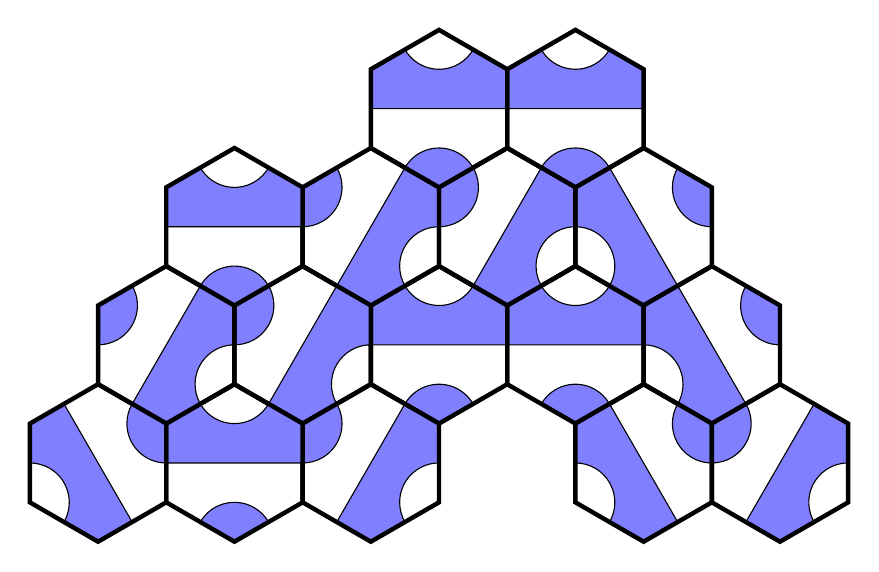
\begin{tikzpicture}[scale=1]
    \foreach \a/\b/\r [evaluate={\a as \x using {\a*sqrt(3)+\b*sqrt(3)/2}}, evaluate={\b as \y using {\b*1.5}}] in {1/-1/0, 1/0/1, 2/-1/1, 2/-2/1, 3/-2/2, 0/1/0, 0/0/2, 0/-1/0, -1/0/2, -1/1/0, -1/-1/2, 0/-2/2, -1/-2/0, -2/-1/2, -2/0/0, -2/-2/1} {
%            3      1       4       1       5      9     2        6       5       3        5       8        9
    % \draw[fill=red!50, rotate around={120*\r:({\x + sqrt(3)/2},{\y + 0.5})}]
    %   ({\x+sqrt(3)},0.5+\y)--
    %   ({\x+sqrt(3)},0+\y)--
    %   ({\x+sqrt(3)/2},-0.5+\y)--
    %   ({\x+0},0+\y)--
    %   ({\x+0},0.5+\y)--
    %   cycle;
    \draw[fill=blue!50, rotate around={120*\r:({\x + sqrt(3)/2},{\y + 0.5})}]
      ({\x+0},0.5+\y)--
      ({\x+0},1+\y)--
      ({\x+sqrt(3)/4},1.25+\y) arc (210:330:0.5)--
      ({\x+sqrt(3)},1+\y)--
      ({\x+sqrt(3)},0.5+\y)--
      cycle;

    % \draw[fill=red!50, rotate around={120*\r:({\x + sqrt(3)/2},{\y + 0.5})}]
    %   ({\x+sqrt(3)/4},1.25+\y) arc (210:330:0.5)--
    %   ({\x+sqrt(3)/2},1.5+\y)--
    %   cycle;

    \draw[fill=blue!50, rotate around={120*\r:({\x + sqrt(3)/2},{\y + 0.5})}]
      ({\x+sqrt(3)/4},-0.25+\y) arc (150:30:0.5)--
      ({\x+sqrt(3)/2},-0.5+\y)--
      cycle;

    \draw[ultra thick]
      ({\x+0},0+\y)--
      ({\x+0},1+\y)--
      ({\x+sqrt(3)/2},1.5+\y)--
      ({\x+sqrt(3)},1+\y)--
      ({\x+sqrt(3)},0+\y)--
      ({\x+sqrt(3)/2},-0.5+\y)--
      cycle;
    }
  \end{tikzpicture}
\end{document}
